% Title: Subset and equality constraints
% Author: Camil Staps
%
% This diagram shows how to use power and sequence types.
\documentclass[border=10pt]{standalone}
\usepackage{tkz-orm}
\begin{document}
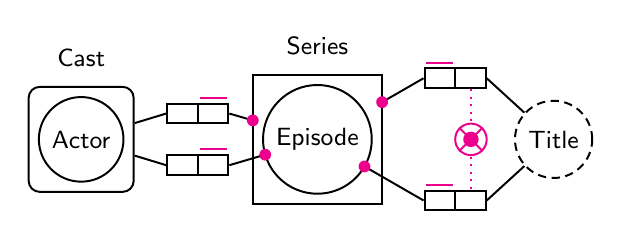
\begin{tikzpicture}[orm-spacious]
    \entity[power=Cast] (actor) at (-3,0) {Actor};
    \entity[sequence=Series] (episode) at (0,0) {Episode};
    \value (title) at (3,0) {Title};

    \binary[below left=of title, unique=1, xshift=-6pt] (et) {};
    \binary[above left=of title, unique=1, xshift=-6pt] (st) {};
    \plays[mandatory] (episode) to (et.west);
    \plays[mandatory] (episode-sequence) to (st.west);
    \plays (title) to (et.east);
    \plays (title) to (st.east);
    \draw[limits] (st.two south) to node[constraint=xor] {} (et.two north);

    \binary[right=of actor-power.south east, unique=2, yshift=10pt] (ec) {};
    \binary[right=of actor-power.north east, unique=2, yshift=-10pt] (sc) {};
    \plays[mandatory] (episode-sequence) to (sc.east);
    \plays[mandatory] (episode) to (ec.east);
    \plays (actor-power) to (sc.west);
    \plays (actor-power) to (ec.west);
\end{tikzpicture}
\end{document}

